% remember to put in tool design
% interview Q's etc - mirror sections from study part 1

To understand how students think about privacy when choosing between VPN
providers, we designed a small-scale lab study.  The results of the interviews
and the survey described in sections~\ref{} suggested that privacy was not of
significant concern to students when choosing a VPN provider to use.
Nonetheless, we wanted to assess if students would value their privacy more if
they were given more information about the privacy practices of VPN providers.
\AH{Should I add a short blurb about what kind of experiment we designed?}

For example, Hotspot Shield--a free VPN
provider--sends data to select trackers through its Chrome
extension~\cite{windscribe-hotspot-shield}. \mc{isn't it also the most popular
vpn, add ref to indicate as much} According to the PAC \mc{describe what this
is for} file in the extension, if an object on a webpage that points to the
domains "analytics.google.com" (owned by Google), "pixel.quantserve.com"
(owned by Quantcast), or "shelljacket.us", then any connections to these
domains are created outside of the VPN.  \AH{Should we show the code for the
PAC file here as a figure?} \mc{yes, show and highlight the relevant piece
with an annotation or caption} This means Google, Quantcast, and Shelljacket can see which
websites users of Hotspot Shield are visiting, even while the users are using
the VPN. \mc{say why this is a data leakage per se}.

\subsection{Method} 

We designed an experiment with Hotspot Shield in which complete a series of tasks while using the VPN. As users complete the tasks, we ask them follow-up questions about their experience using the VPN, and we give them more information about the questionable privacy practices of the VPN. This enables us to answer two questions: 1) do participants care at all about the questionable privacy practices of Hotspot Shield, and 2) what information is most useful to them?

\subsubsection{Surveys and Browser Extension Intervention}

\paragraph{Consent and Baseline Survey.}
Before participating in the study, respondents were asked to fill out a
consent form and a short survey where we collected demographic information.
In the survey, participants confirmed that they have used a VPN before, and
they listed the VPNs they have used in the past.  Participants also gave
consent to audio recording for the experiment.

We also asked the participants several multiple choice questions to elicit
their views on privacy with respect to VPNs.  For example, we asked
participants who they think has access to their data while using a VPN.  We
also asked participants what kinds of data they think are being shared.  These
questions gave us a broad understanding of the views participants had about
VPNs before participating in the experiment.

After the participants completed the pre-study survey, we scheduled times for
each participant to conduct the experiment with a member of the research team.
Each participant again consented to audio recording and confirmed that they
have used a VPN before.  We then explained to the participants that the
purpose of the study was to understand how university students choose between
VPN providers and what factors are most important to them, e.g. ease of use,
privacy, and security.

\paragraph{Background Video and Ratings Survey.}
Once we began recording audio, we asked the participants to watch a short
video on the website for Hotspot Shield about how VPNs work.  We instructed
them to watch this video so that each participant would have a general
understanding of the claims that popular free VPN providers like Hotspot
Shield make with respect to privacy.  After the video ended, we asked the
participants to look around the Hotspot Shield website as they normally would
if they were interested in learning more about the VPN provider.  Once each
participant finished looking around the website, we instructed them to turn on
the Hotspot Shield Chrome extension on their own and configure it to their
liking.

We then gave the participants a set of tasks to complete while Hotspot Shield
was turned on with a research staff member's computer.  These tasks required
the participants to click on links we gave them to find information about
particular things.  In total, there were 3 tasks for each of 3 categories:
entertainment, sexual health, and mental health.  With each task, we
instructed the participants to imagine that they were using their own computer
to find information about something that belonged to these categories.  For
example, one of the tasks for the "sexual health" category reads as follows:
"Imagine that you are interested in learning about the symptoms of Chlamydia.
Visit the following link to find 5 signs of Chlamydia, and write them down."
We also asked the participants to think aloud for the duration of the study,
noting anything that was of interest to them.  \AH{Is there a better way to
tell the reader which tasks we asked the participants to complete?}

Once the participants completed the first set of tasks, we asked them to rate
how likely they would be to use Hotspot Shield on a scale of 1 to 5, with 5
being the highest rating.  At this point in time, the participants were not
informed that Hotspot Shield sends their browsing data to select trackers
outside of the VPN.  Our goal was to gather their thoughts without being
influenced by the privacy practices of Hotspot Shield.

\paragraph{Browser Extension: VPN Audit}
We developed VPN Audit as a Chrome extension to show users the privacy leaks
in Hotspot Shield and design a laboratory study to see how university students
would react.  Figure~\ref{fig:vpn-audit} shows a screenshot of our extension.
The extension works by examining webpages in real time that users visit while
using Hotspot Shield and looking for the Google Analytics, Quantserve, and
Shelljacket trackers.  It then counts the number of unique webpage that these
trackers were present on.  When a user clicks on the name of a tracker, they
see a list of each unique webpage under the "Browsing history sent to tracker"
heading. \mc{need to explain why this is important}


\paragraph{Post-intervention Ratings Survey.}
We then showed the participants VPN Audit before giving them another set of tasks.
At this point in time, we did explain what information the extension was showing because we wanted to see if the participants understood the extension without our intervention.
We simply pointed to the extension, showed them how to access it on their own for the remainder of the experiment, and informed them that it was collecting the displayed information while they were completing the first set of tasks.
The second set of tasks we asked them to complete used the same categories as before: entertainment, sexual health, and mental health.

Once the participants completed the second set of tasks, we asked them to rate how likely they would be to use Hotspot Shield on a scale of 1 to 5, with 5 being the highest rating.
We still did not inform the participants that Hotspot Shield sends their browsing history to select trackers outside of the VPN.
We also did not explain what information VPN Audit was showing them.
Our goal was to see if VPN Audit would change the ratings the participants gave of Hotspot Shield without our intervention.

After the participants gave their ratings for the second time, we explained the privacy practices of Hotspot Shield and explained what information VPN Audit was showing them.
We then showed them an article from The Guardian that explains who Quantserve is and what information they collect through their tracker.
We also showed them an article from Quantserve themselves that explains what information they collect through their tracker.

Finally, we asked the participants one more time to rate how likely they would
be to use Hotspot Shield.  Our goal was to see if participants would change
their ratings again based on all the information we had given them.  We also
asked the participants a set of follow-up questions to gain a deeper
understanding of the reasons behind their ratings.  Lastly, we showed the
participants screenshots of Hotspot Shield's Chrome extension and VPN Audit,
and we asked them to explain and mark up what they saw.  We showed them these
screenshots to gauge their understanding of Hotspot Shield and our tool for
auditing it.



\begin{figure}[t]
    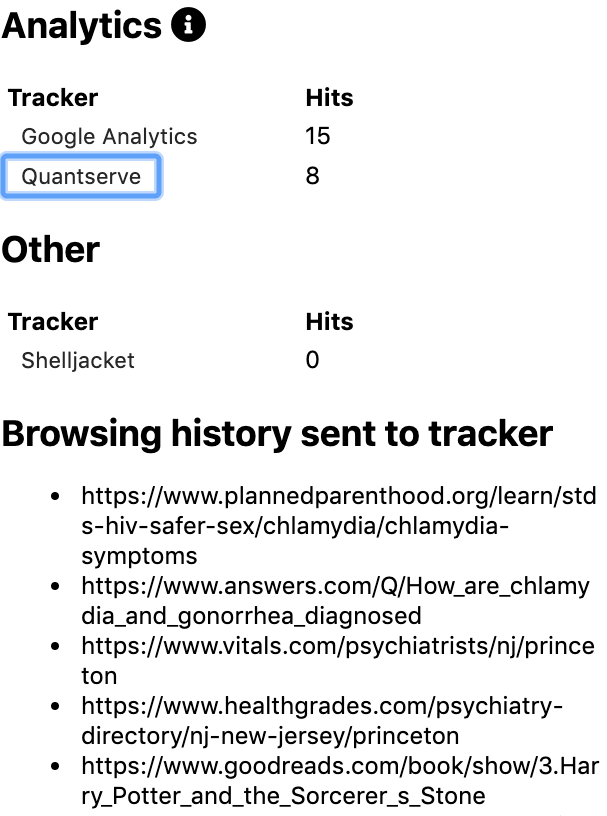
\includegraphics[width=0.85\linewidth]{sections/figures/vpn-audit.png}
    \caption{A screenshot of our Chrome extension for showing the browsing history sent to trackers outside of Hotspot Shield.}
    \label{fig:vpn-audit}
\end{figure}


\subsubsection{Recruitment and Participants} 

We once again recruited participants through listservs maintained by our
institution's survey center.  We filtered for students who had used a VPN
before, who had not participated in the interview or survey studies, and were
currently undergraduate or graduate students at our institution.  All
interviews were audio-taped, and participants were compensated with a \$20
Amazon gift card.

In total, 64 people responded to our recruitment e-mails but some were
ineligible as they had completed the interview or survey or were not students.
We were able to conduct our experiment with 14 of the 65 eligible
participants.  However, we had to discard two interviews owing to audio
related issues and since one of the participants had actually participated in
the survey.  This left us with valid data from 12 participants.

\mc{can we summarize some of this in a table?}
According to the results of our pre-study survey, 9 of our 12 participants were between the ages of 18 and 24 (75\%) and 3 participants were between the ages of 25 and 34 (25\%).
Of these participants, 7 were females (58.3\%), and 5 were males (41.7\%).
Furthermore, 7 of the participants were from the United States (58.3\%), and 5 participants were of other nationalities (41.7\%). 
Lastly, 4 of the participants were computer science students (33.3\%), 3 of the participants were political science students (25\%), and 5 of the participants were studying other majors (41.7\%).

With respect to VPN usage, 8 participants indicated that they have used institutional VPNs (66.7\%), and 3 participants indicated that they have used VPNs that their employers offered (25\%).
Furthermore, 6 participants indicated that they have used a paid, commercial VPN (41.7\%), and 5 participants indicated that they have used a free, commercial VPN (50\%).
Interestingly, 1 participant indicated that they have used a VPN that they set up themselves (8.3\%).

Lastly, with respect to privacy, 10 participants indicated that they have not looked through a VPN provider's privacy policy (83.3\%), with only 2 participants indicating otherwise (16.7\%).
Every participant believed their VPN provider has access to their location (100\%).
Furthermore, 8 of the participants believed their VPN provider collects data about which websites they visit (66.7\%).
Interestingly, 7 of the participants believe VPNs guarantee access to the Internet (58.3\%), 6 of the participants believe VPNs mask their IP address (50\%), and 4 participants believe VPNs guarantee safety from tracking (33.3\%).
However, only 1 participant believes VPNs guarantee anonymity (8.3\%), and only 1 participant believes VPNs guarantee "privacy" (8.3\%).

\subsubsection{Data Processing and Analysis}
We first transcribed the recordings from each session and developed a code book to apply to the transcripts.
Our code book was based on general trends we discovered from an initial reading of the transcriptions.
The codes created related to choosing VPN providers, perceptions of privacy with respect to VPNs, and reactions to VPN Audit.
In total, we created 13 parent codes and 68 child codes. \mc{add example codes} The research team then discussed the coded transcripts and the final themes emerging from the lab sessions are discussed here.

\subsubsection{Limitations}
There are several limitations of our participant demographics that must be considered.
For example, our sample size was limited to 12 participants, which means that our findings cannot generalize to all university students.
Our participants are also mostly Computer Science students that may be more technically sophisticated than students of other disciplines.
Most of our participants are from the United States, which limits our ability to understand how international students think about privacy with respect to VPNs.
Lastly, all of our participants were students at a particular university.

We are also limited by our experiment design in several ways.
Our participants were only exposed to the privacy practices of Hotspot Shield, so we are unable to generalize how they would react to the privacy practices of other VPN providers.
We are also unable to gauge how participants would react to the privacy practices of VPN providers on their own computers and within their own personal space; at best, we can ask them to imagine.
